\chapter{Proposed Work}
\begin{figure*}[h]
    \centering
    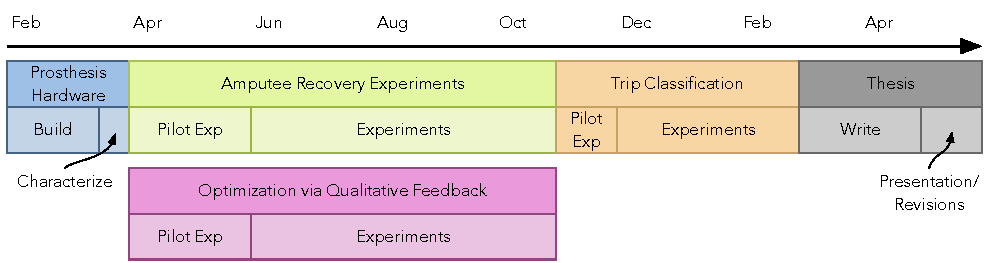
\includegraphics[width=\textwidth]{gantt_chart}
    \caption{Proposed timeline for remaining work.}\label{fig:gantt_chart}
\end{figure*}

\newthought{We investigate two questions} in this thesis: ``Does prosthesis
control based on on a dynamic model of the human neuromuscular system generalize
better to new conditions, resulting in a more robust control?'' And ``can we
improve the control behavior by optimizing its parameters using qualitative
feedback from the amputee?'' To investigate these questions, we propose
completing four tasks before graduation in May 2018: 
\begin{tasks} 
    \item\label{task_1} Build and characterize the performance of our
    transfemoral prosthesis. (\Cref{sec:proposed_build})

    \item\label{task_2} Impose a variety of disturbances to an amputee walking
    on the prosthesis controlled by the Neuromuscular model and assess the
    recovery response. (\Cref{sec:proposed_evaluate})

    \item\label{task_3} Implement a system to optimize control parameters using
    qualitative feedback and evaluate its ability to improve user satisfaction.
    (\Cref{sec:proposed_optimize})

    \item\label{task_4} Improve the existing swing leg control by augmenting it
    with explicit trip detection and execution of recovery strategies.
    (\Cref{sec:proposed_trip_class})
\end{tasks}

\Cref{fig:gantt_chart} shows a Gantt chart that indicates the expected sequence
and duration of these tasks. We expect to complete \cref{task_1} by the end of
April. As \cref{task_2} is largely experimental and will rely on scheduling of
amputee subjects, we expect this task to take nearly a year. In parallel, we
plan to perfom \cref{task_3,task_4}. These two tasks will involve experiments
with non-amputee subjects and thus will be easier to execute.

\section{Build and Characterize Performance of Transfemoral
Prosthesis}\label{sec:proposed_build}

The first step to addressing these questions is to finish construction of the
prosthesis design presented in \cref{sec:completed_design}. So far we have
built, fabricated, and tested the knee joint and fabricated parts for the ankle.
Remaining tasks include assembly of the parts, improving the wiring and cable
management, and implementing a position-control based series elastic control.
The position-based SEA control will command the pre-spring actuator position
$\theta_m$, according to
\begin{align}
    \theta_m = \frac{\tau_d}{k} + \theta_l + \func{PD}{\tau_e} + k_d \omega_l
\end{align}
where $k$ is the series spring stiffness and $k_d \omega_l$ compensates for
damping in the joint. Using a position-based torque control allows us to take
advantage of the fast position control loops of the motor controllers, 
which operate at 5000 Hz versus the 1000 Hz rate of Simulink Realtime. (Compare
to commanding velocity as in the existing control \cref{eq:velocity_based_sea}.)

The preliminary experiments with the active knee joint and passive ankle
prosthesis, shown in
\cref{sec:completed_knee_exp_walk,sec:completed_exp_swing_trip}, suggest the
actuator design seems well suited to the task. However, we have not thoroughly
evaluated the prosthesis performance in terms of step response, bandwidth, and
zero torque tracking. Therefore, we propose to evaluate these characteristics
for both the knee and ankle joints. 

Next, we will evaluate the prosthesis' ability to reproduce walking gait
kinematics and kinetics for steady-state level ground walking. We can quantify
performance in terms of similarity to published steady state walking data of
intact subjects such as that found in \citet{winter2009biomechanics} or
\citet{perry2010gait}. Additionally, we can look for improvement over amputee
subjects' walking gaits when they use their prescribed passive prostheses.
\emph{We estimate that these tasks will take roughly four months to complete.}

\section{Evaluate Neuromuscular Transfemoral Prosthesis
Control Recovery}\label{sec:proposed_evaluate}

We will also investigate the ability of the neuromuscular control to adapt to
novel situations and disturbances. As mentioned in
\cref{sec:back_neuromusc_prosthesis}, previous work on powered ankle prostheses
has demonstrated neuromuscular control adapts to slopes by producing more torque
when walking up slopes and less when walking down slopes
\citep{eilenberg2010control} and adapts to changes in speed by producing more
ankle plantarflexion work as gait speed increases \citep{markowitz2011speed}. As
the knee joint is governed by similar force feedback reflexes, and is linked to
the ankle via the biarticular gastrocnemius muscle, we expect the knee joint to
show similar increases in output. \citet{chen1997influence} show that the knee
indeed significantly increases its power output as incline or speed increase.
Similarly, \citet{mcintosh2006gait} find that the knee produces significantly
higher knee flexion moment at heel strike on downward inclines and significantly
higher knee extension moment at the end of double stance on upward inclines.

More generally, we expect the neuromuscular model to adapt well to novel
circumstances because it encodes key features of walking mechanics such as the
role of positive force feedback and the damping effect of muscle's
force-velocity relationship in generating stable compliant leg behavior
(\citep{grey2007positive} see \cref{sec:neuro_hill_muscle}), the importance of
biarticular structures for preventing joint overextension during leg compression
\citep{seyfarth2001stable}, and the need for swing control to achieve target
foot placements. To empirically test the contribution of these mechanisms to
stabilizing gait, we also propose to subject amputees to disturbances such as
sudden treadmill speed changes and impulses applied to the amputee's hip by the
PushBot Robot. We can quantify the responses in terms of the time required to
regain normal gait and compare to the response of impedance control. \emph{We
expect this task to take roughly ten months to complete.}

\section{Optimizing Prosthesis Control using Qualitative
Feedback}\label{sec:proposed_optimize}

In the discussion of our current method for optimizing control parameters
(\cref{sec:tuning_discussion}), we identified several possible improvements.
One possible change is to allow more varied qualitative feedback that such as
absolute good/bad ratings, unsure preferences, and ``better than all'' feedback.
We can easily incorporate this feedback into the GP framework by amending
\cref{eq:likelihood} with additional terms. For absolute good/bad ratings we can
incorporate the likelihood function used in GP classification to categorize
points as either ``good'' or ``bad'' \citep{williams2006gaussian}. For points
belonging to the good class, the likelihood takes the form
\begin{align}
    \prob{D_{n_\tn{g}}^\tn{g}|\vecf{f}} &= 
        \prod_{k=1}^{n_\tn{g}} \prob{\textsc{isGood}(x_k)| f(x_k)} 
        = \prod_{k=1}^{n_\tn{g}} \Phi(q_k^\tn{g}),
    \label{eq:likelihood_abs_good}
\end{align}
where $D_{n_\tn{g}}^\tn{g} = \{x_1, \ldots, x_k, \ldots, x_{n_\tn{g}}\}$ is the
set of points the user has classified as good and $q_k^\tn{g} =
\frac{f(x_k^\tn{a})}{\sigma_\tn{g}}$. The likelihood has the effect of pushing
the function values for points classified as good higher, with parameter
$\sigma_\tn{g}$ controlling the strength of this effect. We can define an
analogous likelihood function $\prob{D_{n_b}^\tn{b}|\vecf{f}}$ for points the
user identifies as bad.

If the user identifies two points that he or she is unsure of the preference
between, we can utilize a likelihood function that pulls the function values of
the two points closer together. Given a data set of ambiguous or ``unclear''
relations $D_{n_\tn{u}}^\tn{u} = \{x_1^\tn{a} \simeq x_1^\tn{b}, \ldots,
x_k^\tn{a} \simeq x_k^\tn{b}, \ldots, x_n^\tn{a} \simeq x_n^\tn{b}\}$ (where
$\simeq$ denotes approximate equality of latent function value), we can use the
likelihood
\begin{align}
    \prob{D_{n_\tn{u}}^\tn{u}|\vecf{f}} &= \prod_{k=1}^{n_\tn{u}} \prob{x_k^\tn{a}
        \simeq x_k^\tn{b} | f(x_k^\tn{a}), f(x_k^\tn{b})} 
        = \prod_{k=1}^{n_\tn{u}} \mathcal{N}(q_k),
    \label{eq:likelihood_unclear}
\end{align}
where $\mathcal{N}(\cdot)$ is the standard normal distribution.

Finally, we can easily incorporate ``better than all seen so far'' feedback as
preferences between that point and all other points seen so far. We can then
replace the likelihood in the posterior distribution (\cref{eq:bayes_rule}) with
the product of the likelihoods of all forms of feedback.

To incorporate time adaptation into the model, we can simply add time as a
dimension to all points. In a Gaussian Process, the kernel function governs the
correlation between the function value of a point in the training dataset and
the function value of a new test point. The Gaussian kernel we currently employ,
decreases the correlation between points as the euclidean distance between them
increases. Therefore, appending the time to all data points will diminish the
effect of old data points on new predictions.

We will test this improved method for learning from qualitative feedback in two
scenarios both involving real user feedback. In the first scenario, we project
foot placement targets onto a treadmill and users are asked to walk while
hitting the target on every step. The target placement is governed by up to five
parameters: width, skewness, frequency, and left and right foot direction. Users
will provide their qualitative feedback on these parameters and we will gauge
how fast the system converges to the user's preferred foot placement parameters.
In this case, we can assume users prefer zero skewness, and straight foot
placement. We can measure their step frequency beforehand, and hand-tune the
width. We choose this scenario as it has a clear optimum that we can find easily
via hand tuning. We can perform this optimization in one, three, and five
dimensions to assess how the algorithm scales as dimensionality increases.  In a
second scenario, we apply the method to tune the parameters of the prosthesis
stance control. We then look for improvement over the default control parameters
and for local optimality by comparing to points near the identified optimum.
\emph{We will perform this task in parallel with the neuromuscular control task
over the course of five months (see \cref{fig:gantt_chart}).}

\section{Learning Trip Recovery Policies}\label{sec:proposed_trip_class}

In the final proposed work, we plan to investigate methods for detecting and
recovering from stumbles during swing. As mentioned earlier, recovery during
mid-swing disturbances seems to be an issue for the current control
architecture.  Appropriately dealing with these disturbances will likely require
explicit detection, classification, and execution of a recovery strategy.
Previous work in this area has trained classifiers on data obtained by tripping
healthy human subjects \citep{lawson2010stumble, shirota2014recovery}. The
authors then evaluate these classifiers via offline cross validation, in which a
subset of the training data is set aside and used for testing, and report low
error-rates. 

However, directly applying classifiers trained on healthy human subjects to
detect and respond to trips on the prosthesis may result in poor performance as
it would violate the i.i.d.\ assumptions of the trained classifiers.  This is
because when we trip an amputee wearing the prosthesis, the generated
distribution of data will differ from that generated by tripping a healthy
subject. Moreover, once the classifier makes a mistake in responding to a
disturbance, which is already more likely, the generated data will look even
less like the training data resulting in even further degraded performance. 

Unfortunately, we also cannot initially gather data from an amputee wearing the
prosthesis, as this would require a working trip classifier and recovery
strategy, which is what we are trying to achieve in the first place. This
chicken or the egg problem has been identified previously in the imitation
learning literature. To solve this problem, \citet{ross2011reduction} propose a
training method based on \emph{dataset aggregation} (Dagger). In this method, we
train the classifier and then execute it on the real system. We then label the
resulting data, augment the original training dataset with the new data, and
repeat this procedure iteratively. In this way, we can ensure that the policy is
trained on the data it will itself generate and that the classifier learns to
recover from its own mistakes. With this training procedure I believe we can
successfully implement active trip recovery strategies on the powered
prosthesis.

\begin{marginfigure}
    \centering
    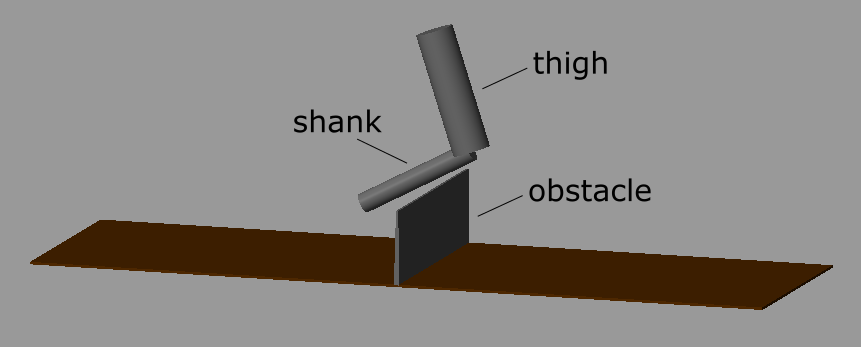
\includegraphics[width = \linewidth]{trip_sim.png}
    \caption{Swing leg model used to train and test trip detection
    SVM.}\label{fig:trip_sim}
\end{marginfigure}
We tested in simulation the hypotheses that online error rates will be greater
than offline error rates when we use classifiers to control the swing leg trip
response and that employing Dagger training improves trip classification error
rates. To do this we modeled a swing leg in the Simulink Simscape Multibody
Environment (\cref{fig:trip_sim}). We controlled by a heuristic ``expert''
policy that can perfectly identify impacts with obstacles and then
stochastically chooses to execute either a raising or lowering strategy. Using
kinematic data generated by 25 executions of the expert policy, we trained two
SVMs: one that distinguishes between unimpeded swing and disturbed swing and one
that, when the first SVM detects a trip, classifies the response as either a
raising or lowering strategy. As shown in \cref{fig:dagger_result}, the offline
error rates, evaluated when the expert policy still controls the swing leg, are
very small, $0.50\%$ and $0.00\%$ respectively. However, when we evaluate these
classifiers in the online-case, where the trained policies control the system,
we see much higher error rates of $20.7\%$ and $29.3\%$ respectively. Finally,
employing the Dagger method to train the system. In this case we first use the
expert policy to generate 5 trajectories and train the to SVMs. We then use the
SVMs to control the system and generate 5 new trajectories and retrain the
classifiers.  We repeat this 3 more times so that in total there are 25
trajectories in the dataset. With this method, the online error rates are
$0.02\%$ and $12.0\%$ for the trip detection and strategy classification SVMs
respectively. 
\begin{marginfigure}[-1in]
    \centering
    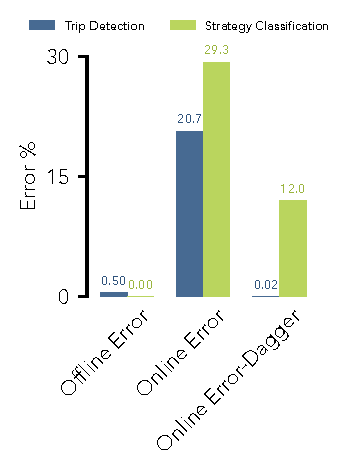
\includegraphics[width = \linewidth]{dagger_result}
    \caption{Online error rates of trip detection and classification SVMs are
    significantly higher than offline error rates. Using a Data set aggregation
    approach helps reduce the online error rate.}\label{fig:dagger_result}
\end{marginfigure}

We can employ a similar training method to improve trip detection and strategy
identification on the real prosthesis. For the initial trip detection policy, we
can programmatically engage the trip recovery controller when the trip is
applied by PushBot. For the initial strategy classification policy, we can use
policies trained on healthy subjects, or have an operator visually classify the
amputee's response and select the correct recovery response in real-time. We can
then iteratively train classifiers and execute them on the system to gather more
training data. At the end of the procedure, we can evaluate the classifier error
rates, and compare against controllers trained only using the response of
healthy subjects. \emph{We expect this task to take roughly four months to
complete in parallel with the amputee experiments of \cref{task_2}.  (see
\cref{fig:gantt_chart}).}

\section{Proposed Work Summary}\label{sec:proposed_summary}

Our proposed tasks seek to address the three challenges of amputee locomotion we
identified in the introduction (\cref{sec:intro_challenges}). Namely, that it is
a dynamic task requiring consideration of interaction forces with the
environment and obstacles, that it requires a control that is robust to changes
in gait and disturbances, and that amputees are unique and require
individualized control parameters. 

We propose to address these challenges through four main contributions: First,
we design and characterize a series elastic prosthesis design capable of
executing dynamic locomotion tasks. Second, we implement and characterize
prosthesis control based on a neuromuscular model of human locomotion. In
simulation, such models have proven to be robust to disturbances, and previous
experiments with powered ankle prostheses have demonstrated that they can adapt
to amputee gait variations such as speed and incline changes. Third, we propose
to improve upon the existing control structure by implementing specific reflexes
that respond to mid-swing disturbances. Finally, we intend to adapt the
neuromuscular control parameters to individual subjects by using their
qualitative feedback and preferences between control parameter sets.

If these tasks are completed successfully, the resulting prosthesis design and
control strategy should significantly improve transfemoral amputee gait
robustness, while still providing a natural and individualized nominal gait. As
we noted in the introduction (\cref{sec:intro_motivation}), transfemoral
amputees face a variety of gait deficits and are often unable to complete many
tasks such as walking on uneven terrain, walking without support, and walking
with loads. While we will not have completely addressed all these deficits, we
will have hopefully provided evidence for a promising direction for continued
research that will eventually fully address these issues. 
